\begin{figure}[H]
\centering
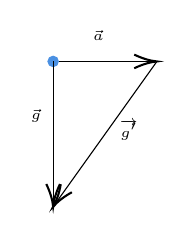
\begin{tikzpicture}[x=0.75pt,y=0.75pt,yscale=-1,xscale=1]
%uncomment if require: \path (0,300); %set diagram left start at 0, and has height of 300

%Straight Lines [id:da6000594042392968] 
\draw    (280,88) -- (328,88) ;
\draw [shift={(330,88)}, rotate = 180] [color={rgb, 255:red, 0; green, 0; blue, 0 }  ][line width=0.75]    (10.93,-3.29) .. controls (6.95,-1.4) and (3.31,-0.3) .. (0,0) .. controls (3.31,0.3) and (6.95,1.4) .. (10.93,3.29)   ;
%Shape: Circle [id:dp5092551209319207] 
\draw  [color={rgb, 255:red, 74; green, 144; blue, 226 }  ,draw opacity=1 ][fill={rgb, 255:red, 74; green, 144; blue, 226 }  ,fill opacity=1 ] (282.5,88) .. controls (282.5,86.62) and (281.38,85.5) .. (280,85.5) .. controls (278.62,85.5) and (277.5,86.62) .. (277.5,88) .. controls (277.5,89.38) and (278.62,90.5) .. (280,90.5) .. controls (281.38,90.5) and (282.5,89.38) .. (282.5,88) -- cycle ;
%Straight Lines [id:da48222497169597345] 
\draw    (280,88) -- (280,156) ;
\draw [shift={(280,158)}, rotate = 270] [color={rgb, 255:red, 0; green, 0; blue, 0 }  ][line width=0.75]    (10.93,-3.29) .. controls (6.95,-1.4) and (3.31,-0.3) .. (0,0) .. controls (3.31,0.3) and (6.95,1.4) .. (10.93,3.29)   ;
%Straight Lines [id:da2944838205191447] 
\draw    (330,88) -- (281.16,156.37) ;
\draw [shift={(280,158)}, rotate = 305.54] [color={rgb, 255:red, 0; green, 0; blue, 0 }  ][line width=0.75]    (10.93,-3.29) .. controls (6.95,-1.4) and (3.31,-0.3) .. (0,0) .. controls (3.31,0.3) and (6.95,1.4) .. (10.93,3.29)   ;

% Text Node
\draw (298,72) node [anchor=north west][inner sep=0.75pt]  [font=\tiny] [align=left] {$\displaystyle \vec{a}$};
% Text Node
\draw (268,110) node [anchor=north west][inner sep=0.75pt]  [font=\tiny] [align=left] {$\displaystyle \vec{g}$};
% Text Node
\draw (311,115) node [anchor=north west][inner sep=0.75pt]  [font=\tiny] [align=left] {$\displaystyle \overrightarrow{g^{\prime }}$};


\end{tikzpicture}
    \caption{存在恒加速}
\end{figure}